%% This is file `elsarticle-template-2-harv.tex',
%%
%% Copyright 2009 Elsevier Ltd
%%
%% This file is part of the 'Elsarticle Bundle'.
%% ---------------------------------------------
%%
%% It may be distributed under the conditions of the LaTeX Project Public
%% License, either version 1.2 of this license or (at your option) any
%% later version.  The latest version of this license is in
%%    http://www.latex-project.org/lppl.txt
%% and version 1.2 or later is part of all distributions of LaTeX
%% version 1999/12/01 or later.
%%
%% The list of all files belonging to the 'Elsarticle Bundle' is
%% given in the file `manifest.txt'.
%%
%% Template article for Elsevier's document class `elsarticle'
%% with harvard style bibliographic references
%%
%% $Id: elsarticle-template-2-harv.tex 155 2009-10-08 05:35:05Z rishi $
%% $URL: http://lenova.river-valley.com/svn/elsbst/trunk/elsarticle-template-2-harv.tex $
%%

%%\documentclass[preprint,authoryear,12pt]{elsarticle}

%% Use the option review to obtain double line spacing
%% \documentclass[authoryear,preprint,review,12pt]{elsarticle}

%% Use the options 1p,twocolumn; 3p; 3p,twocolumn; 5p; or 5p,twocolumn
%% for a journal layout:

%% Astronomy & Computing uses 5p
%% \documentclass[final,authoryear,5p,times]{elsarticle}
\documentclass[final,authoryear,5p,times,twocolumn]{elsarticle}

%% if you use PostScript figures in your article
%% use the graphics package for simple commands
%% \usepackage{graphics}
%% or use the graphicx package for more complicated commands
\usepackage{graphicx}
%% or use the epsfig package if you prefer to use the old commands
%% \usepackage{epsfig}

%% The amssymb package provides various useful mathematical symbols
\usepackage{amssymb}
%% The amsthm package provides extended theorem environments
%% \usepackage{amsthm}

\usepackage[pdftex,pdfpagemode={UseOutlines},bookmarks,bookmarksopen,colorlinks,linkcolor={blue},citecolor={green},urlcolor={red}]{hyperref}
\usepackage{hypernat}

%% The lineno packages adds line numbers. Start line numbering with
%% \begin{linenumbers}, end it with \end{linenumbers}. Or switch it on
%% for the whole article with \linenumbers after \end{frontmatter}.
%% \usepackage{lineno}

%% natbib.sty is loaded by default. However, natbib options can be
%% provided with \biboptions{...} command. Following options are
%% valid:

%%   round  -  round parentheses are used (default)
%%   square -  square brackets are used   [option]
%%   curly  -  curly braces are used      {option}
%%   angle  -  angle brackets are used    <option>
%%   semicolon  -  multiple citations separated by semi-colon (default)
%%   colon  - same as semicolon, an earlier confusion
%%   comma  -  separated by comma
%%   authoryear - selects author-year citations (default)
%%   numbers-  selects numerical citations
%%   super  -  numerical citations as superscripts
%%   sort   -  sorts multiple citations according to order in ref. list
%%   sort&compress   -  like sort, but also compresses numerical citations
%%   compress - compresses without sorting
%%   longnamesfirst  -  makes first citation full author list
%%
%% \biboptions{longnamesfirst,comma}

% \biboptions{}

\journal{Astronomy \& Computing}

\begin{document}

\begin{frontmatter}

%% Title, authors and addresses

%% use the tnoteref command within \title for footnotes;
%% use the tnotetext command for the associated footnote;
%% use the fnref command within \author or \address for footnotes;
%% use the fntext command for the associated footnote;
%% use the corref command within \author for corresponding author footnotes;
%% use the cortext command for the associated footnote;
%% use the ead command for the email address,
%% and the form \ead[url] for the home page:
%%
%% \title{Title\tnoteref{label1}}
%% \tnotetext[label1]{}
%% \author{Name\corref{cor1}\fnref{label2}}
%% \ead{email address}
%% \ead[url]{home page}
%% \fntext[label2]{}
%% \cortext[cor1]{}
%% \address{Address\fnref{label3}}
%% \fntext[label3]{}

\title{Automated reduction of submillimetre single-dish heterodyne
  data from the James Clerk Maxwell Telescope using ORAC-DR}

%% use optional labels to link authors explicitly to addresses:
%% \author[label1,label2]{<author name>}
%% \address[label1]{<address>}
%% \address[label2]{<address>}

\author[jac]{Malcolm J.\ Currie\corref{cor1}}
\ead{m.currie@jach.hawaii.edu}
\author[jac,cornell]{Tim Jenness}
\ead{tjenness@cornell.edu}
\author[jac]{Remo P.\ J.\ Tilanus\fnref{rpt}}
\author[jac]{Brad Cavanagh}
\author[jac]{David S. Berry}
\author[jac]{Jamie Leech\fnref{jxl}}
\author[jac]{Luca Rizzi\fnref{lr}}

\cortext[cor1]{Corresponding author}
\fntext[rpt]{Present address: Leiden Observatory, PO Box 9513, 2300 RA
  Leiden, The Netherlands}
\fntext[jxl]{Present address: Department of Physics, University of
  Oxford, Denys Wilkinson Building, Keble Road, Oxford, OX1 3RH, UK}
\fntext[lr]{Present address: W.\ M.\ Keck Observatory, 65-1120 Mamalahoa Hwy, Kamuela,
  HI 96743, USA}

\address[jac]{Joint Astronomy Centre, 660 N.\ A`oh\=ok\=u Place, Hilo, HI
  96720, USA}
\address[cornell]{Department of Astronomy, Cornell University, Ithaca,
  NY 14853, USA}

\begin{abstract}
%% Text of abstract

With the advent of modern multi-receptor heterodyne instruments that
can result in observations generating thousands of spectra per minute it is
no longer feasible to reduce these data as individual spectra. This
paper describes how baselined, mosaicked data cubes can be created by
an automated pipeline in a reliable manner, including detection of bad
spectra, removal of transient effects and creation of high fidelity
moment maps.

\end{abstract}

\begin{keyword}
%% keywords here, in the form: keyword \sep keyword

%% MSC codes here, in the form: \MSC code \sep code
%% or \MSC[2008] code \sep code (2000 is the default)

submillimeter astronomy \sep
methods: data analysis \sep
pipelines \sep
techniques: spectroscopic \sep
techniques: image processing \sep
James Clerk Maxwell Telescope

\end{keyword}

\end{frontmatter}

% \linenumbers

%% Journal abbreviations
\newcommand{\mnras}{Mon Not R Astron Soc}
\newcommand{\aap}{Astron Astrophys}
\newcommand{\pasp}{Pub Astron Soc Pacific}
\newcommand{\apj}{Astrophys J}
\newcommand{\qjras}{Quart J R Astron Soc}
\newcommand{\an}{Astron.\ Nach.}
\newcommand{\ijimw}{Int.\ J.\ Infrared \& Millimeter Waves}

%% Applications
\newcommand{\makecube}{\textsc{Makecube}}

%% main text
\section{Introduction}
\label{sec:intro}

As heterodyne receivers have progressed from single-receptor
instruments
\citep{1992IJIMW..13.1487P,1992IJIMW..13..647D,1992IJIMW..13.1827C} to
small focal plane arrays
\citep{2003SPIE.4855..322G,2004A&A...423.1171S} to 16 element arrays
such as HARP at JCMT \citep{2009MNRAS.399.1026B}, and beyond
\citep{2007stt..conf..264G}, and correlators have improved such that
we can easily obtain spectra at 10\,Hz with 8192 channels, data rates
have increased substantially such that it is now common-place to take
a short observation resulting in thousands of spectra. This is only
going to become worse with the advent of instruments with 64,000
channels and large format arrays such as CHAI on CCAT
\citep{2009ASPC..417..113R}.

In submillimeter astronomy data reductions packages such as
\htmladdnormallinkfoot{CLASS}{http://www.iram.fr/IRAMFR/GILDAS} and
SPECX \citep{SPECX} were developed that worked well with
single-receptor instruments. Scripting interfaces and tools for
curating collections of spectra were insufficient as the data rates
increased and data pipelines were suggested
\citep[e.g.,][]{1995ASPC...75..117W}. The ACSIS data reduction system
\citep{2000ASPC..216..502L,2000SPIE.4015..114H}, delivered to the JCMT
in 2005, aimed to deal with the data rate issues by providing a
pipeline that sent the calibrated spectra, with optional baselining,
to a component that would place the spectra in to a data
cube. Although it was possible to store the raw data in CASA
measurement sets \citep{2012ASPC..461..849P}\footnote{At the time this
  was being developed CASA was known as AIPS++}, the data cube was the product that was archived and
taken away by the astronomer for further analysis. This strategy was
forced on us given the computer resources available when ACSIS was
being designed and developed and was known to have risks associated
with it. Coadding spectra into the cube allowed for impressive ``data
compression'' for stare and jiggle observing modes although the gains
were much less in scanning observing modes. There were many downsides
though. The observing system required that the cube parameters be
specified and initially it was felt that the observer should select
the parameters in the Observing Tool \citep{2002ASPC..281..453F}. It
was also necessary that the observer specify the baseline regions and
any frequency binning required. The gridding and the frequency binning
were irreversible and the observer needed to ensure they did not make
a mistake. Additionally, baselining with anything other than a DC
offset was also problematic as the fit parameters for every spectrum
were not stored and so could not be reversed. The burden placed on the
observer having to specify everything, whilst simultaneously not
making a mistake, was not acceptable and by 2006 we realised that
computers were fast enough and storage large enough to be able to
write the calibrated spectra directly to disk and defer further data
reduction to a pipeline.

\section{Heterodyne Data Reduction Pipeline}

It was decided that data reduction recipes would be written for the
existing ORAC-DR pipeline infrastructure in use at JCMT
\citep{TFAJenness2011,2008AN....329..295C} with key requirements that
the output data cube should be specified from the telescope pointing
information and the location of each receptor on the sky, and that
baseline regions should be determined automatically by examining the
spectra as an ensemble. Furthermore, as progress was made on the
pipeline we additionally realised that we should also be able to
detect bad spectra and remove them from the coadd as well as doing
quality assurance tests. The latter were critical for the JCMT Legacy
Survey projects
\citep{2007PASP..119..855W,2009ApJ...693.1736W,2007PASP..119..102P}
who wanted to ensure they received data of consistent quality.

The JCMT heterodyne pipeline has two operating modes. The default behaviour is
for the pipeline to generate the best possible data products without
regard to efficiency. This is generally what is required by scientists
at their institutions and the mode we run in at the JCMT Science
Archive \citep{2008ASPC..394..565J}. The other mode is a cut-down
version of the recipes that runs at the JCMT itself during
observing. This pipeline has constrained timing requirements and can
not perform many of the advanced processing features provided by the
main pipeline. It's role is to provide simple quality assurance
information and basic coadds to the observer and it will not be
discussed further in this paper.

\subsection{Determining Cube Parameters}

Once we decided that we would not require that a PI specifies their
pixel grid in advance, it became clear that we would have to provide
software that would automatically determine the pixel grid from the
data itself. In the SMURF package data cubes are created from
calibrated spectra using the \makecube\ command. \makecube\ can be
given an externally specified grid but also has an \texttt{autogrid}
option that leaves optimal grid determination to the application itself.

Autogrid first projects the supplied sky positions into pixel
positions using an arbitrary tangent plane projection that has
1~arcmin square pixels with North upwards and the target position
(or the first supplied sky position if no target position is
available) at pixel (1,1).

It then projects each of these pixel positions onto a straight line
passing through pixel (1,1) at an angle, theta, to North. This line is
divided up into sections of length 1~arcmin, and a histogram formed
of the number of projected positions that fall in each section. The
amplitude and wavelength of any periodicity in this histogram is found
by looking at the auto-correlation of the histogram (the amplitude is
the auto-correlation at zero shift, and the wavelength is the shift at
the first significant peak in the auto-correlation function).

This is repeated for many different line orientations in order to find
the value of theta (line orientation) that gives the strongest
periodicity in the histogram. This orientation is used as the
direction for the X pixel axis in the final grid. The corresponding
wavelength is used as the pixel spacing on the X axis. The wavelength
of the periodicity perpendicular to his direction is then found and
used as the pixel spacing on the Y axis.

FInally, we shift the reference pixel coordinates by up to one pixel
on each axis in order to minimise the sum of the squared distances
from each pixel projected sample position to the nearest pixel centre.

\textit{Is there anything else in makecube that we want to mention
  that contributes to the automated processing?}

\subsection{Sub-band merging}

\textit{Anything to say here?}

\subsection{Automated Baseline Removal}

The real meat: smoothing, basic baseline subtraction, group coadd,
clump finding, unmakecube, source masking, iteration.

\begin{figure}
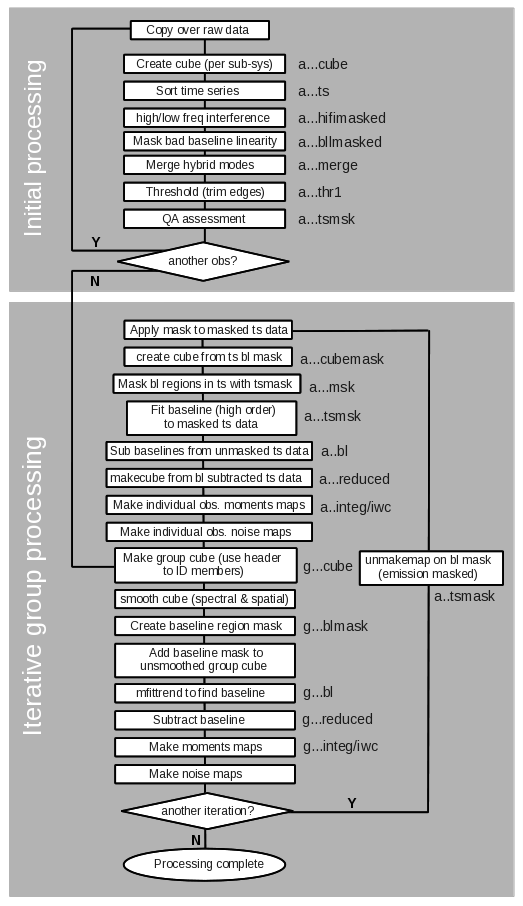
\includegraphics[width=90mm]{flowchart.png}
\caption{Flow chart of the pipeline recipe. This is currently Holly's
  figure and needs to be redone for the paper (at least to be in
  scalable form) or else we ask Holly if we can use it. Placeholder
  for now.}
\label{fig:flowchart}
\end{figure}

\subsection{Determination of moment maps}

Moment maps can be compromised if excessive baseline is included in
the calculation. For example, in an integrated intensity calculation
the inclusion of all the baseline noise can hide a weak line. The data
reduction system has already calculated where the baseline regions are
for each spectrum and so for moment maps this mask is negated. This
leads to much improved fidelity.

\textit{Figure of integrated intensity image with masking compared to
  one without the baseline masking}

\subsection{Removal of Bad-Baseline Spectra}



\textit{Malcolm's ADASS XXII poster and JCMT Newsletter article. Blog mentions
that we might also handle ringing in spectra.}

The bad baselines can be divided roughly into two classes:
high-frequency, high amplitude; and low frequency, lower
amplitude. The former appear mostly in single isolated spectra or in
narrow bands, but can also manifest as spiky spectra, or
weaker-amplitude striations persistent over tens of spectra.
Figure~\ref{fig:badbase:highfreq} presents the most-common forms.

\begin{figure}[!ht]
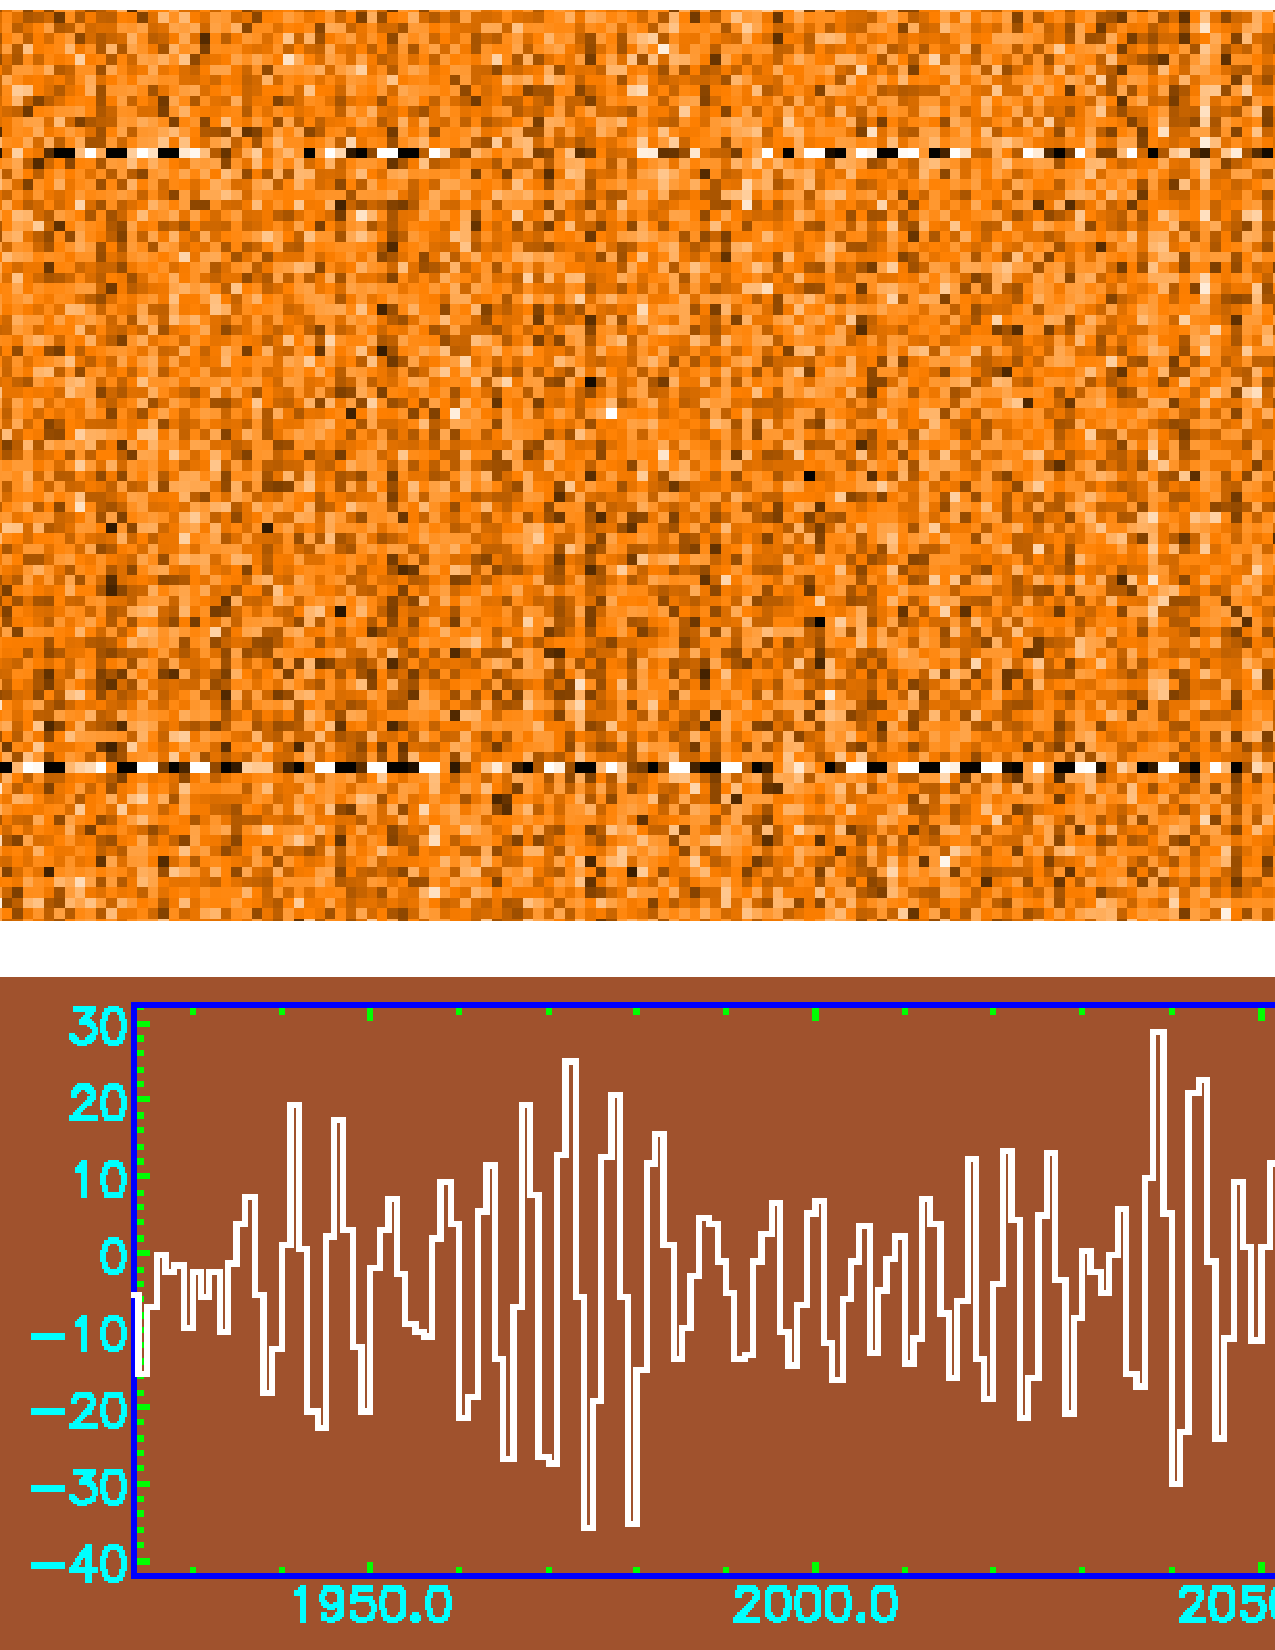
\includegraphics[width=0.23\textwidth]{P61_f1a}
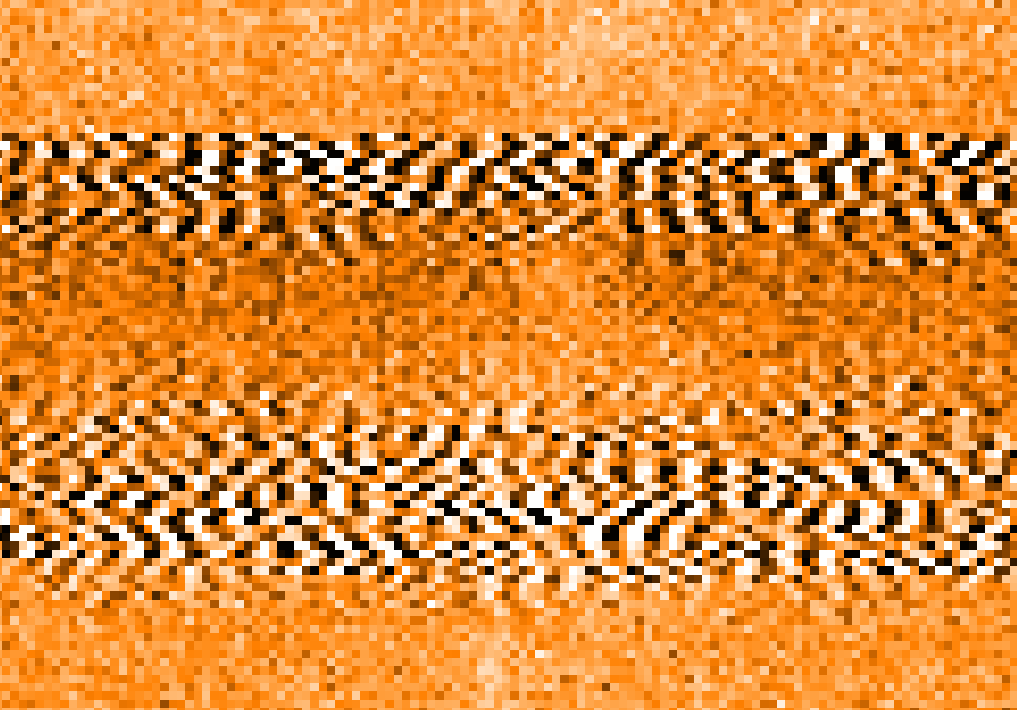
\includegraphics[width=0.23\textwidth]{P61_f1b}
\caption{Examples of high-frequency interference in spectral-time
  axes. The left panel shows high-amplitude interference affecting
  single spectra; and part of an affected spectrum plotted below. The
  amplitude dwarfs the normal signal by an order of magnitude. The
  right panel shows bands of phase-shifting interference.}
\label{fig:badbase:highfreq}
\end{figure}

The low-frequency ripples tend to occur in time-series blocks that are
often visible because of baseline drift, but can apply to all spectra
for a receptor. They have a wide range of morphologies such as
sinusoids, irregular ripples, and curved, twin headlight-like beams
that start strong but gradually pan out and fade with time.
Figure~\ref{fig:badbase:interference} displays some examples.

\begin{figure}[!ht]
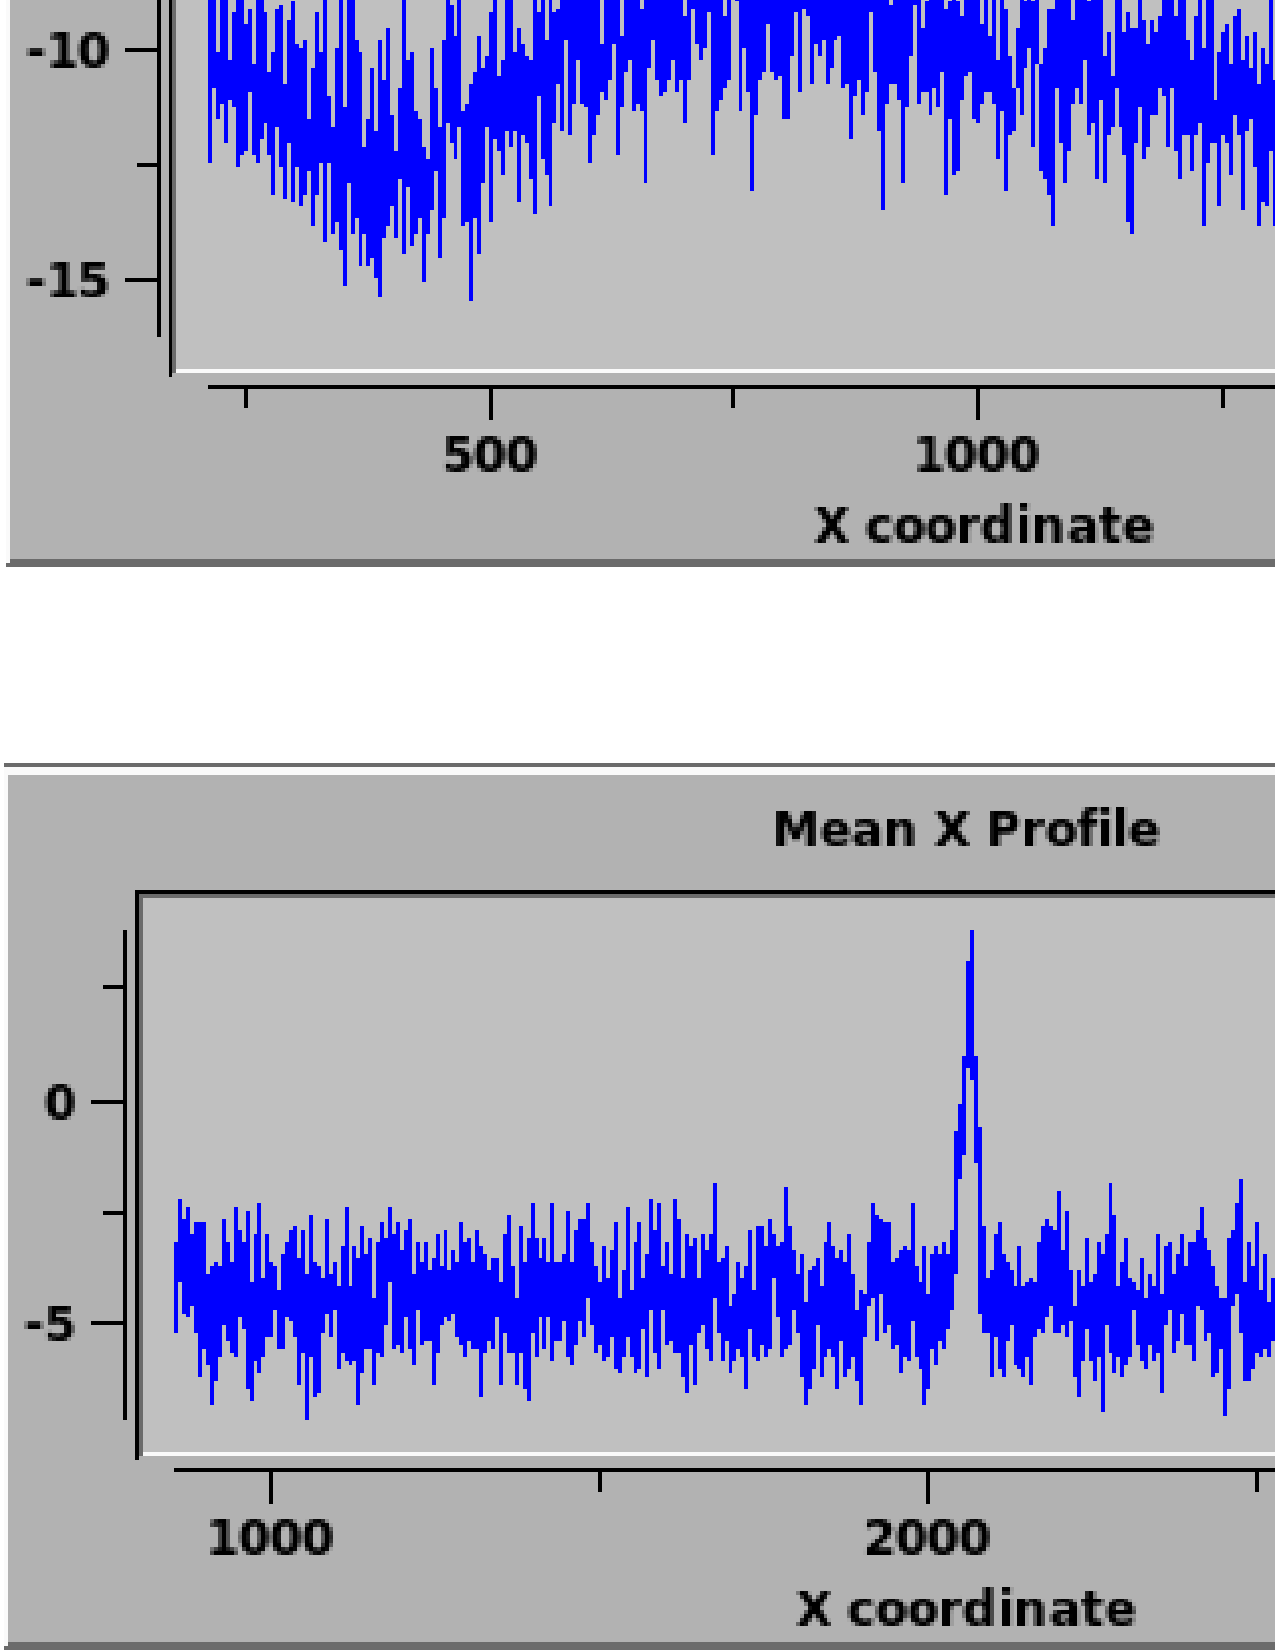
\includegraphics[width=0.23\textwidth]{P61_f2a}
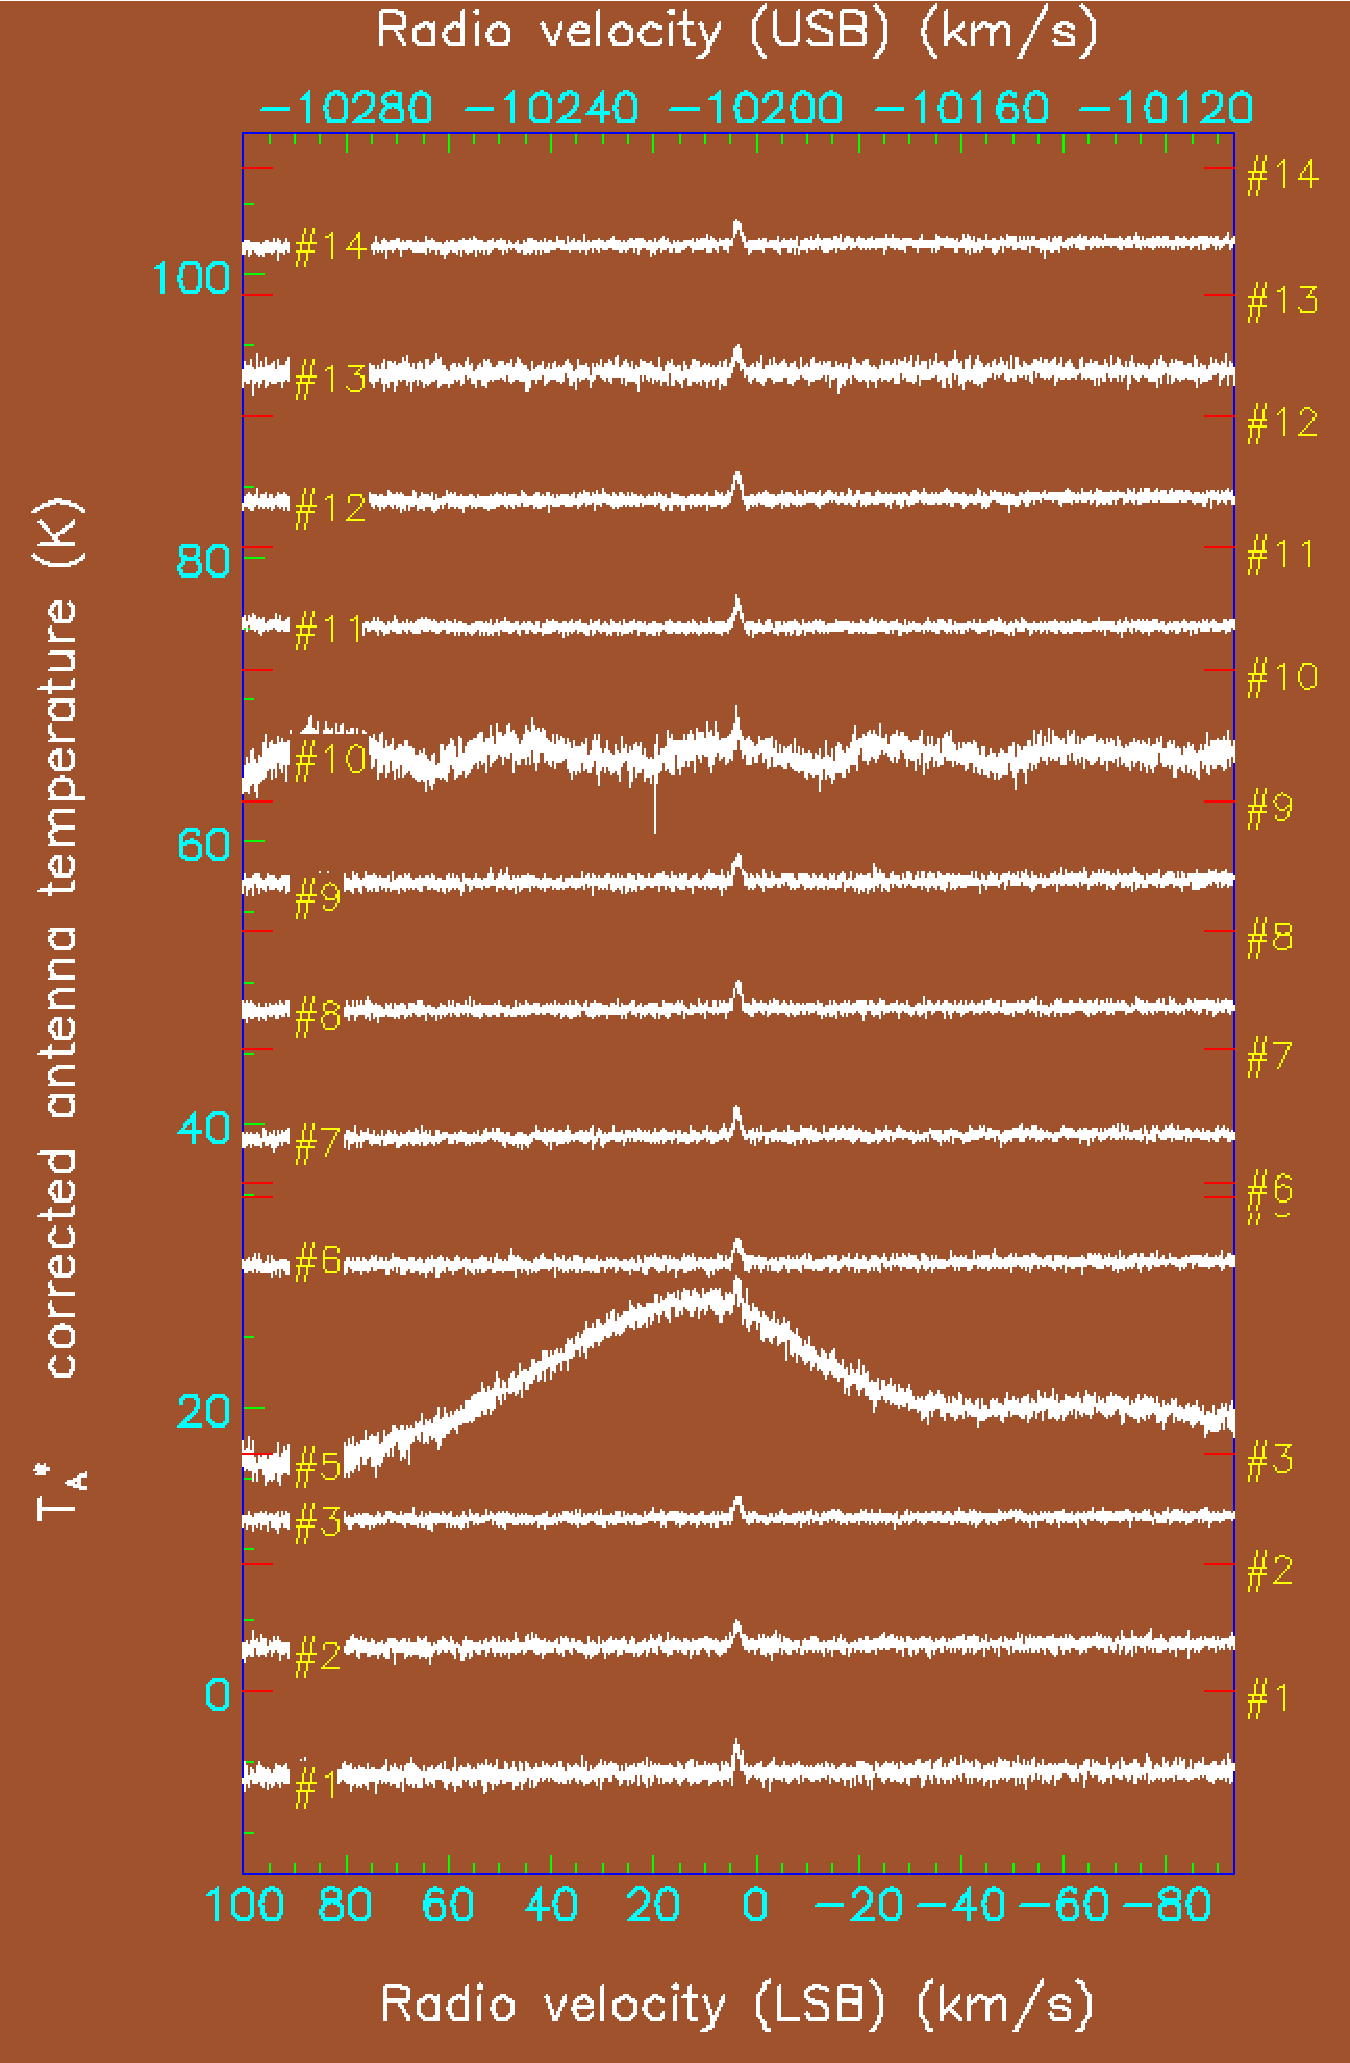
\includegraphics[width=0.23\textwidth]{P61_f2b}
\caption{Examples of low-frequency interference.  The top-left graphic
  shows a band of low-frequency oscillations; below it is the band's
  average spectrum.  The lower-left spectrum has a periodic weak
  ripple hard to detect visually.  The right panel shows time-averaged
  (clipped mean) spectra for each receptor in which the fourth and
  ninth from the bottom exhibit global non-linearity.}
\label{fig:badbase:interference}
\end{figure}

\subsubsection{Adopted solution}

The pipeline applies three steps in the quality-assurance stage:
\begin{itemize}
\item Laplacian filtering of high-frequency noise
\item non-linearity detection for individual spectra
\item global non-linearity to reject whole receptors
\end{itemize}

\subsubsection{Masking of High-Frequency Noise}

The recipe applies a one-dimensional Laplacian edge filter to all the
spectra for each receptor trimming the outer 15~\% where noise is
always present.  This approximates to a difference-of-Gaussian
filter. It next sums the rms `edginess' along the spectral axis to
form a profile through the time series.  Drifts or steps in the
profile are removed.  The final step is to eject spectra whose rms
edginess exceeds the median level by a nominated number of clipped
standard deviations.  Affected spectra are easily delineated.  An
optional second iteration removes most of the striation noise once the
pronounced edginess peaks are masked.

\subsubsection{Non-linearity Filtering}

The low-frequency rippled and wobbly baselines are addressed by
determining the non-linearity of each spectrum.  First the recipe
excludes non-baseline features that would dilute the non-linearity
signal.  These comprise a threshold to remove spikes and masking a
central region where the astronomical signal may be present. It
estimates the background level, effectively smoothing to remove
structure smaller than a nominated scale.  Next it fits linear
baselines to these and calculates the rms residuals to provide a
rectified signal.  Then it averages the signal along the spectral axis
to form a non-linearity profile through the time series for each good
receptor.

The non-linear profiles are much noisier than the summed Laplacians
and discrimination is harder.  To identify anomalous spectra the
recipe reduces the noise to obtain a smooth profile, correct for
drifts or steps in the profile.  It rejects spectra whose mean
non-linearity exceeds the mean level above a nominated number of
clipped standard deviations.  The derived standard deviation allows
for positive skewness.  It applies a mask of rejected spectra to the
input cube.

The global non-linearity test is applied last so that a block of
transient highly deviant spectra will not cause the whole receptor to
be rejected.  It operates in a similar fashion to the above.  It
diverges by determining a mean rms residual from non-linearity per
detector, from which it evaluates the median and standard deviation of
the distribution of mean rms residuals from the entire observation,
and performs iterative sigma clipping above the median to reject those
detectors whose deviations from linearity are anomalous.  There is a
tunable minimum threshold.

\subsubsection{Results}

The methods appear highly effective at cleaning the pipeline
products. It has been used to re-reduce one survey and several other
datasets. Figure~\ref{fig:badbase:results} presents an example which
had originally failed quality assurance, but now can be used for
science.

\begin{figure}
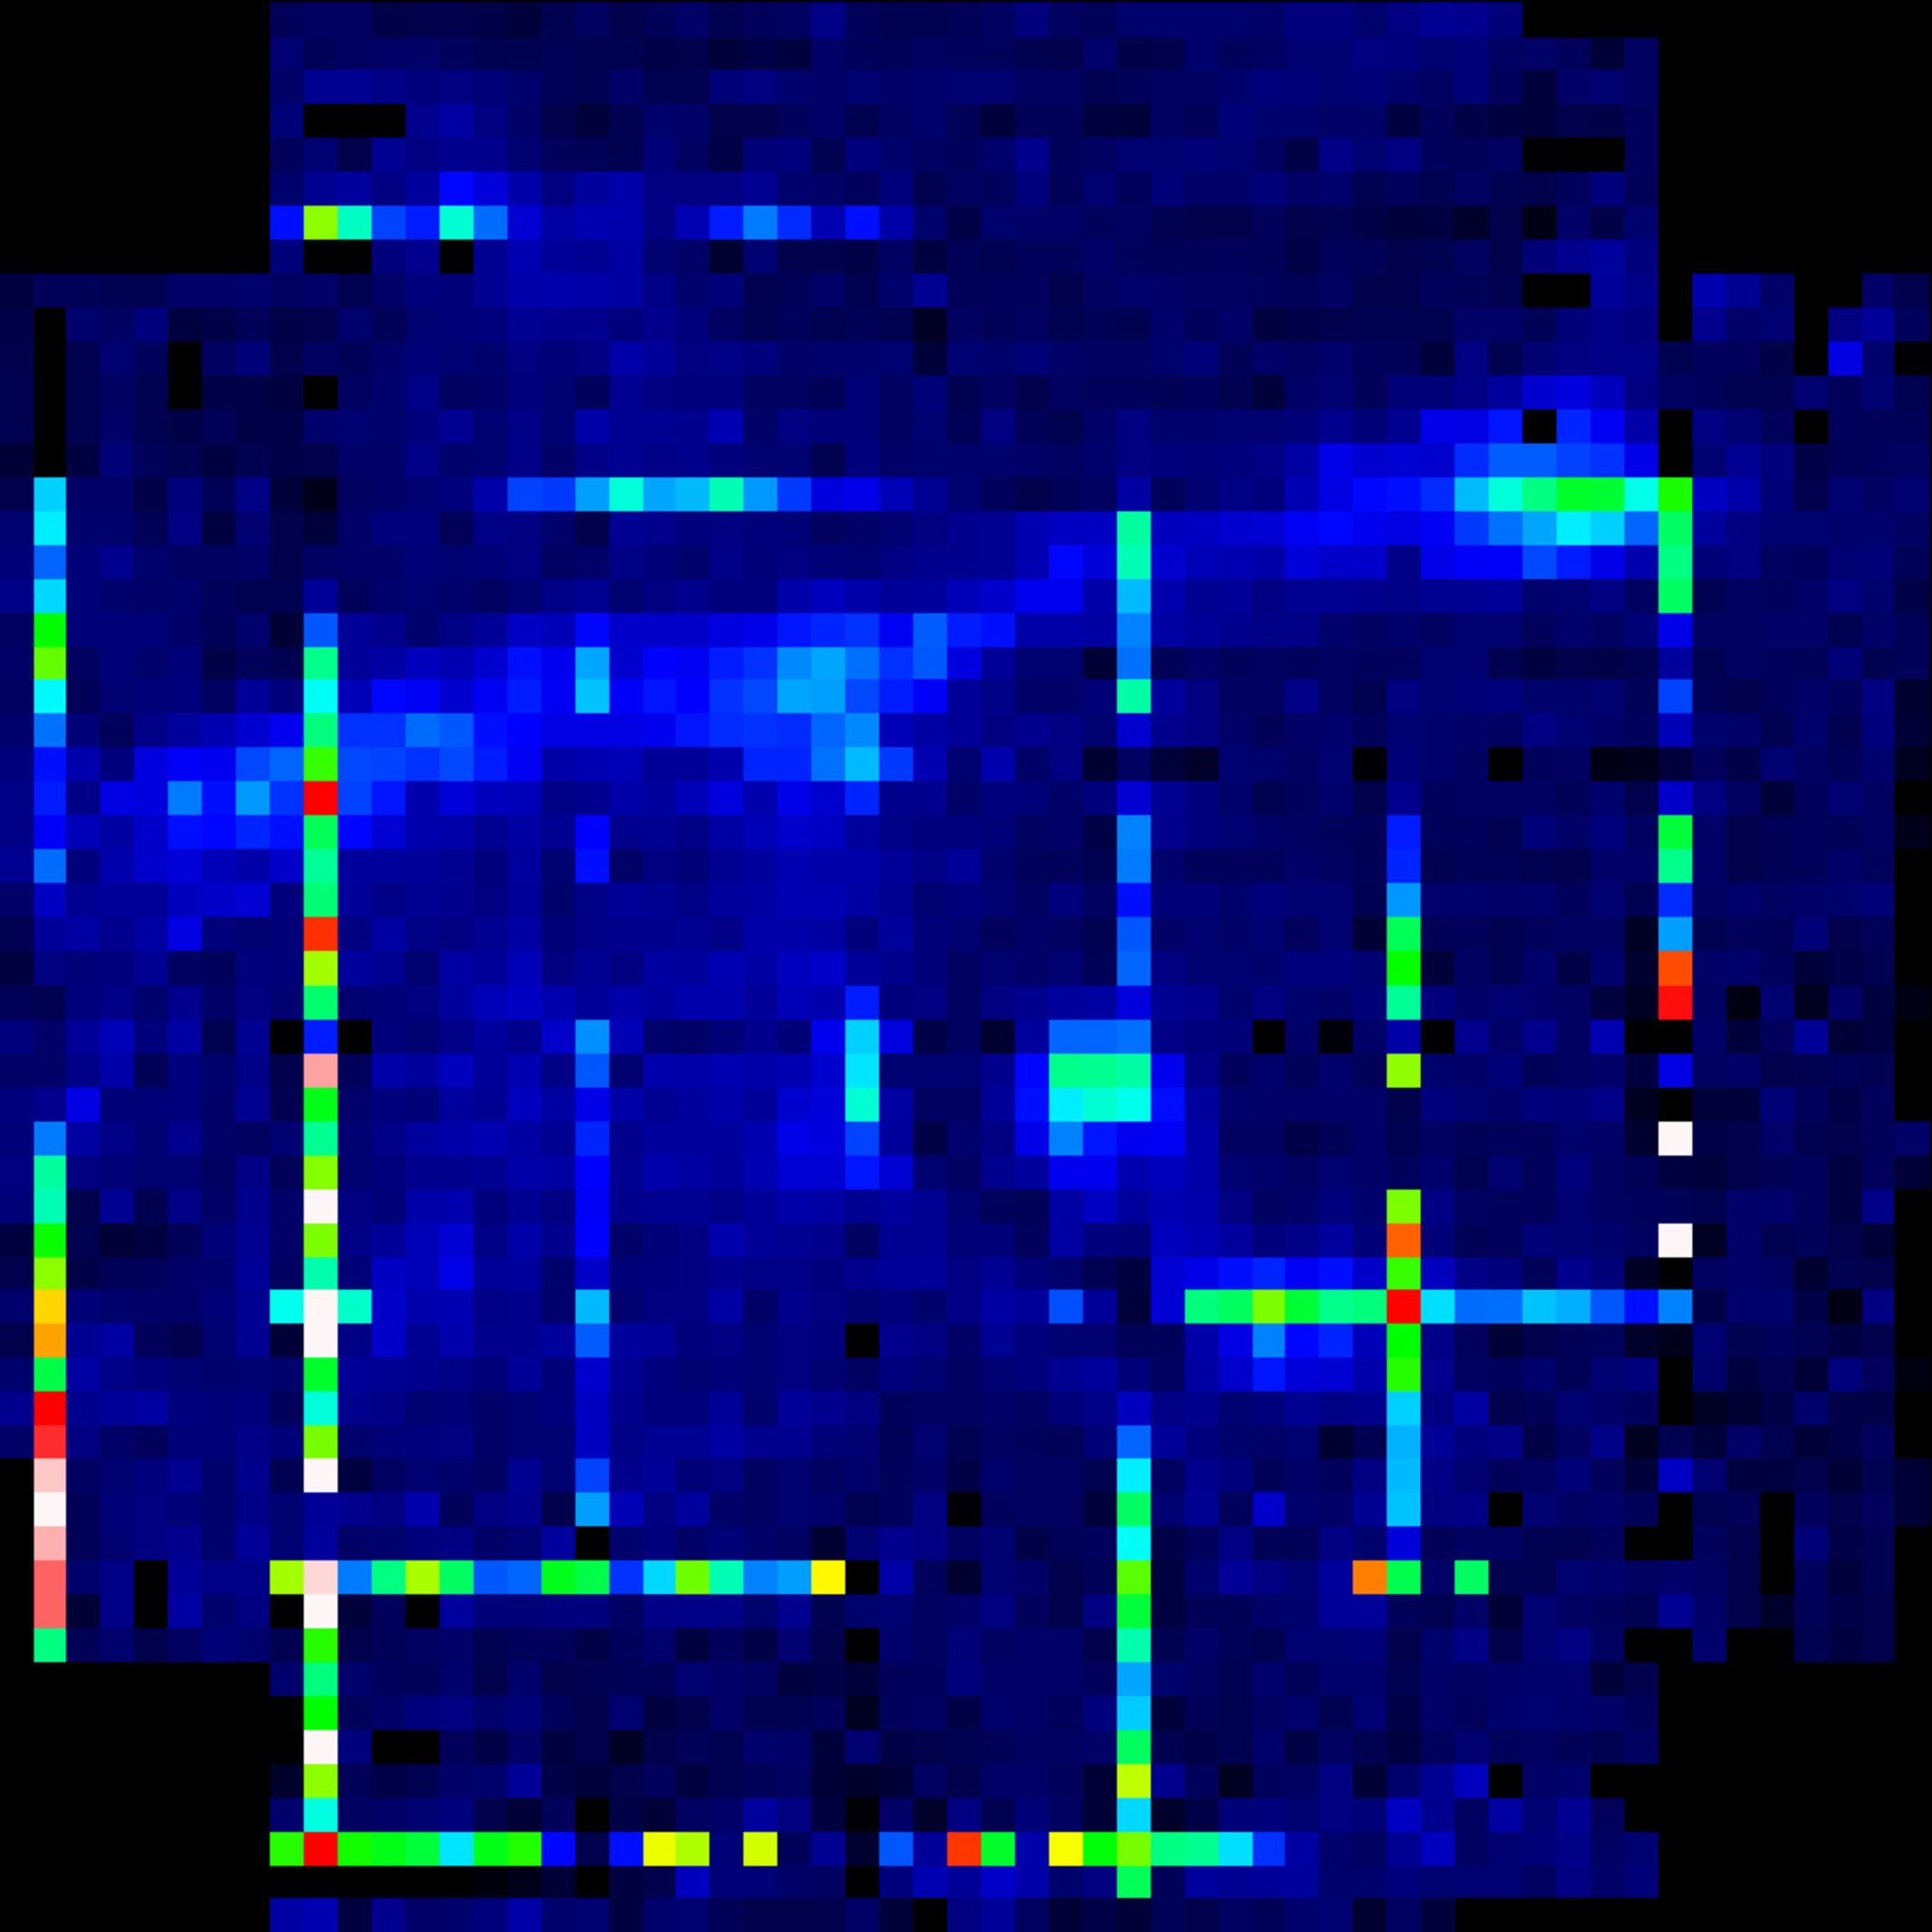
\includegraphics[width=0.23\textwidth]{P61_f3a}
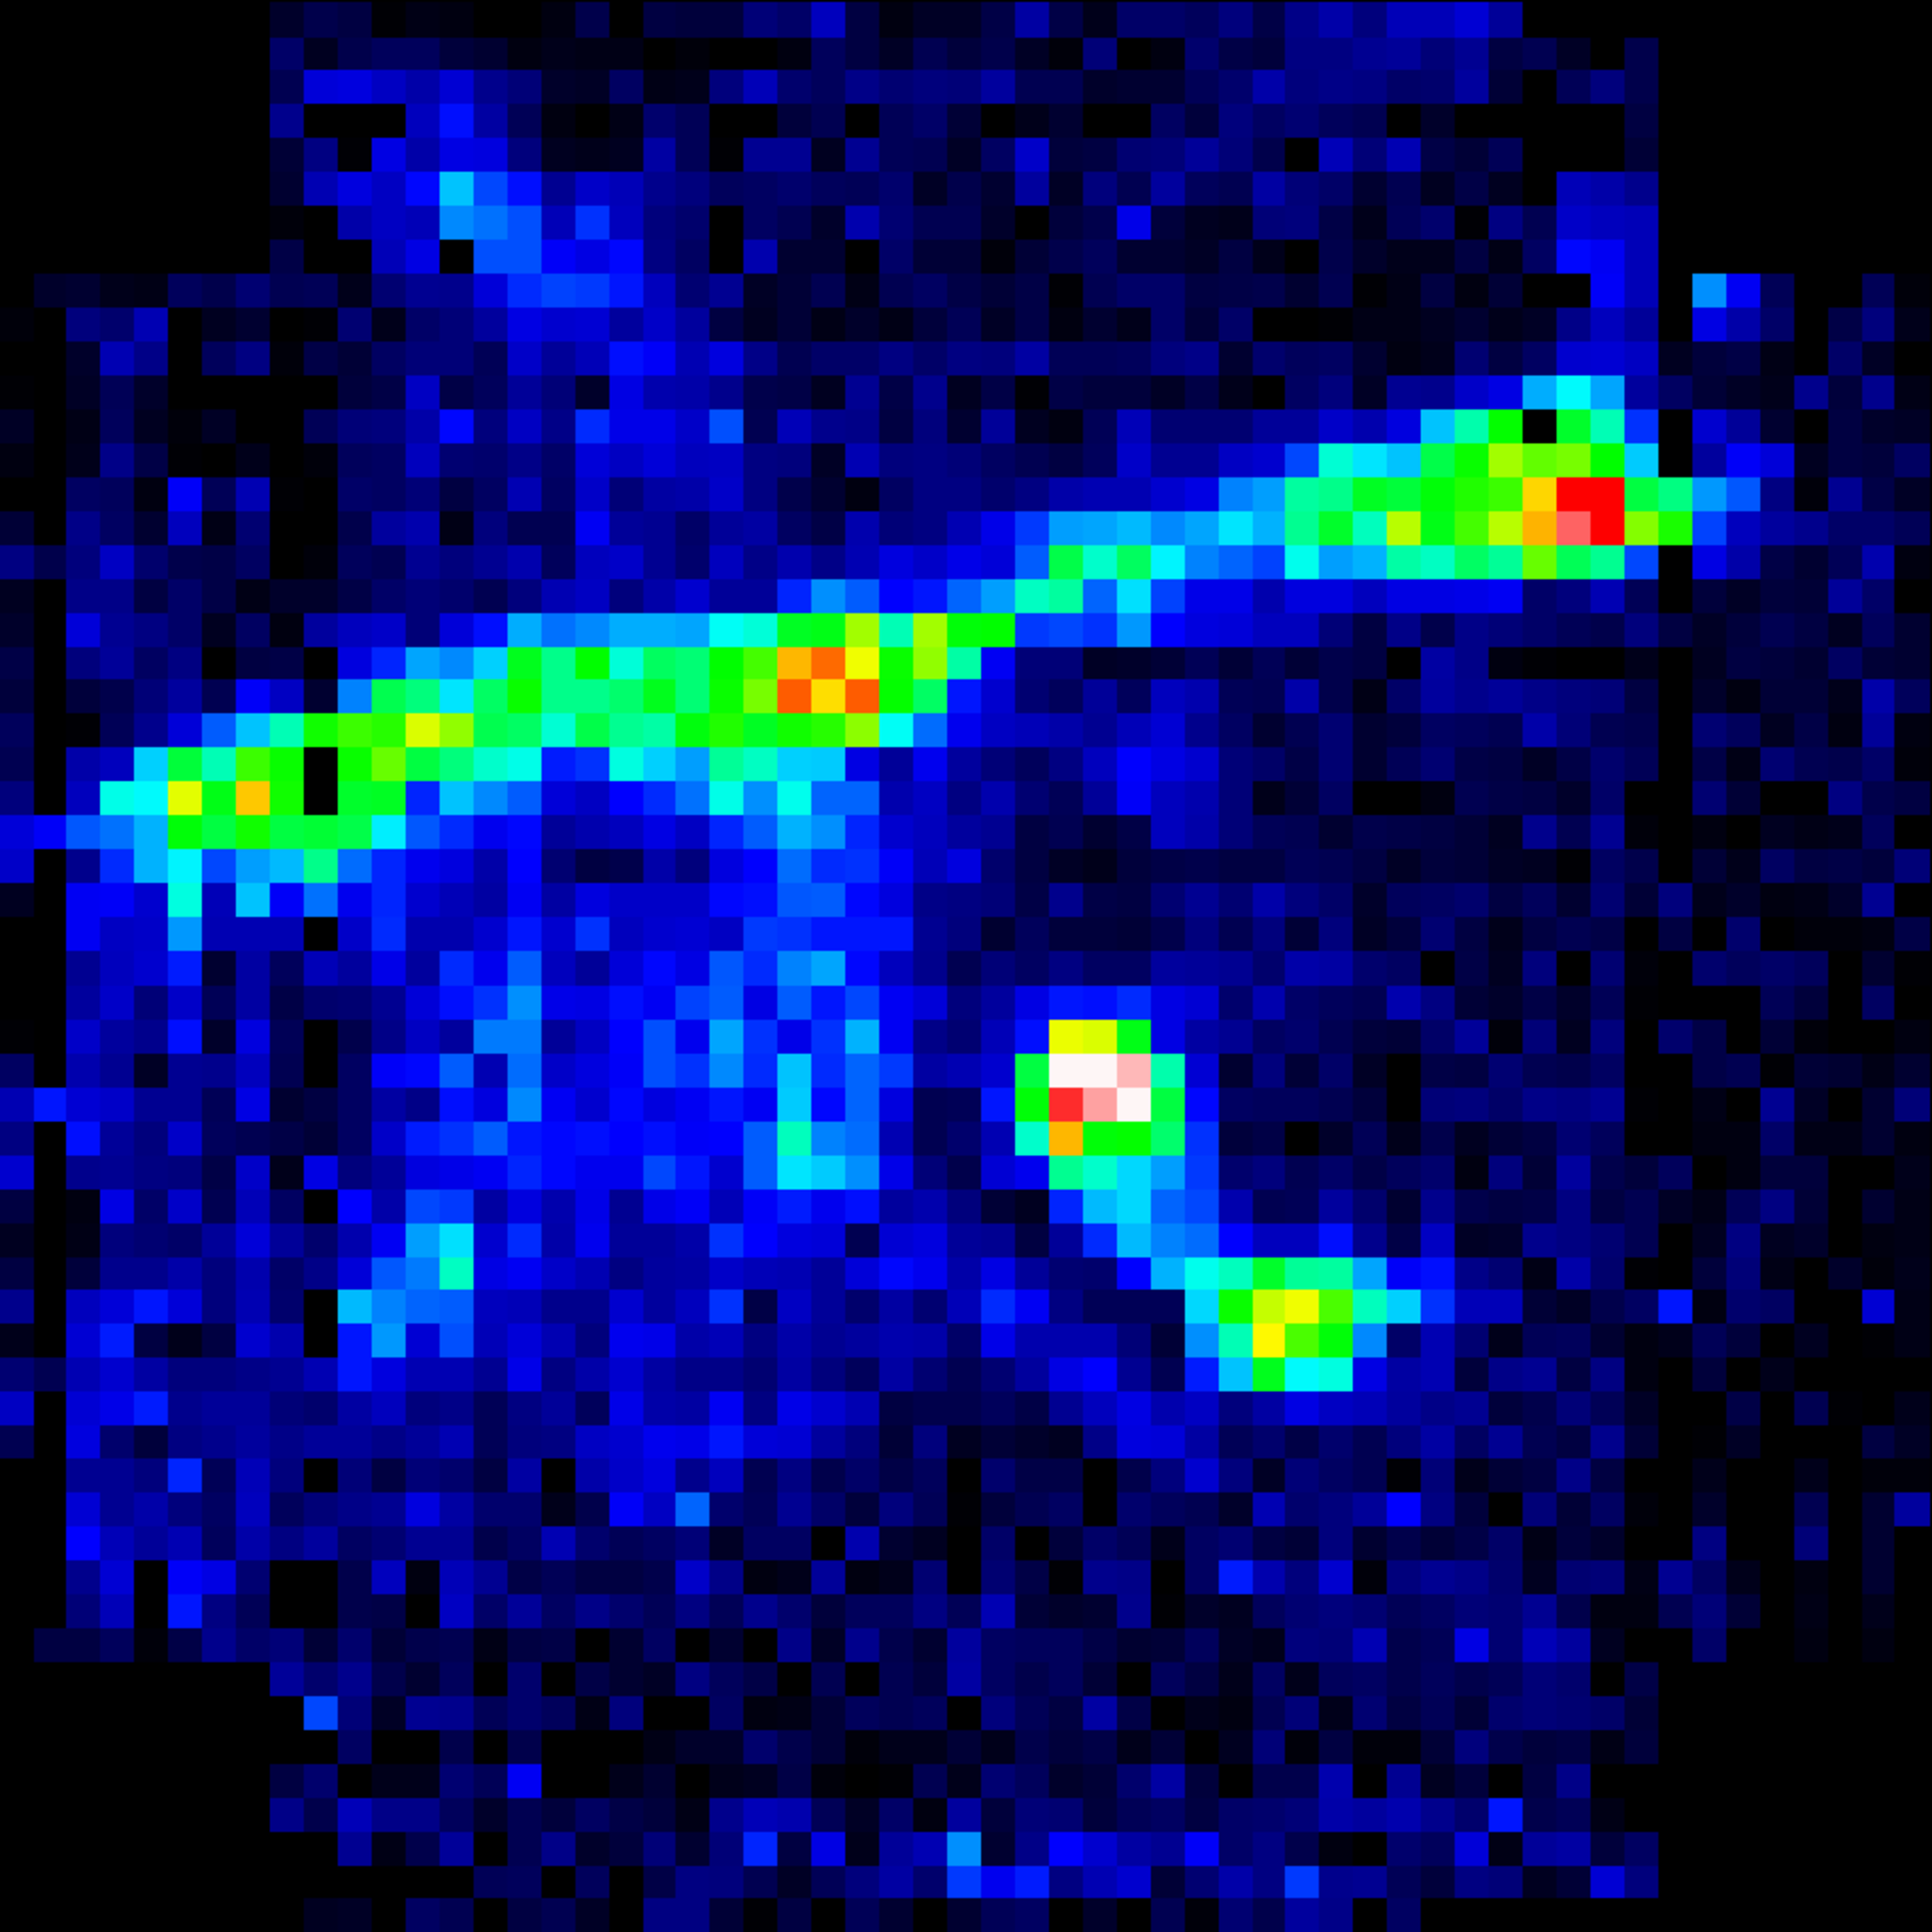
\includegraphics[width=0.23\textwidth]{P61_f3b}
\caption{Comparison of an integrated intensity map using the same
  percentile scaling.  The left panel shows a map without bad-baseline
  removal.  The right panel shows the same data processed using the
  new filters.}
\label{fig:badbase:results}
\end{figure}

\subsection{Flatfielding}

Early HARP data from 2006 seemed to have problems with the relative
calibration of the receptors. A self flatfielding algorithm was
developed that relied on the receptors on average seeing the same
signal for large scan maps of molecular clouds
\citep{2010MNRAS.401..455C} and this had some success in removing
striping from integrated intensity images.

Now discuss the pipeline implementation. Before and after flatfielding examples.

\subsection{Recipe Tuning}

The data reduction system can be configured by using recipe parameters
supplied to ORAC-DR in a file. Each recipe has its own set of
parameters that are supported and these can include options to bin up
the frequency scale, control the output grid, control and regridding
parameters and enable or disable flatfielding and bad baseline filtering.

\subsection{Quality Assurance Parameters}

The survey teams required a comprehensive set of quality assurance
testing to ensure that the data quality is consistent. A number of QA
tests were added and a full list is shown in Table \ref{tab:qa:params}.

\begin{table}
\caption{Quality Assurance Parameters}
\label{tab:qa:params}
\begin{tabular}{ll}
BADPIX\_MAP  & \\
CALINTTOL & \textit{Not implemented?} \\
CALPEAKTOL & \textit{Not implemented?} \\
FLAGTSYSBAD & \textit{Not implemented?} \\
GOODRECEP & \textit{Not implemented?} \\
RESTOL & \textit{Not implemented?} \\
RESTOL\_SM & \textit{Not implemented?}  \\
RES\_CHAN & \textit{Not implemented?}  \\
RMSMEANTSYSTOL & \\
RMSTSYSTOL & \\
RMSTSYSTOL\_FAIL & \\
RMSTSYSTOL\_QUEST & \\
RMSVAR\_MAP & \\
RMSVAR\_RCP &  \textit{Not implemented?} \\
RMSVAR\_SPEC & \\
TSYSBAD &  \textit{Not implemented?} \\
TSYSMAX &  \textit{Not implemented?} \\
TSYSVAR &  \textit{Not implemented?} \\
VELRES
\end{tabular}
\end{table}

\subsection{Alternative Recipes}

It is not possible or even desirable for a single data reduction
technique to apply to many different types of sources and science
goals. For that reason a number of different recipes are made
available and these can be chosen by the observer in the Observing
Tool, overridden later on the command-line or by using a
configuration file at the JCMT Science Archive.

\subsubsection{Gradient}

This is the standard recipe optimized for nearby molecular clouds with
relatively narrow lines where there can be a velocity gradient across
the cloud. This velocity gradient is a major motivation for the
automated detection of baseline regions as it allows you to maximize
the baseline region rather than supplying a simple range that
encompasses all the data.

\subsubsection{Broad line}

Nearby galaxies have broad lines of many km/s so this recipe is tuned
to be less aggressive for automatic baseline subtraction than the
standard recipe that is deisgned for nearby molecular clouds.

\subsubsection{Line Forest}

Some transitions are very close together, for example methanol, and
different techniques are required for handling the automated basline
subtraction.

\textit{Do we use findback?}

\subsubsection{Continuum}

For continuum observations, such as planets, baseline subtraction
should not be done.

\subsubsection{Frequency Switch}

\section{Processing of Legacy Data}

Until ACSIS was delivered in 2005, heterodyne data were taken with a
variety of backend systems including the Acousto-Optical Spectrometer
(AOSC) and the Dutch Autocorrelation Spectrometer (DAS)
\citep{1986SPIE..598..134B}. These backends wrote data in the
Global Section Data (GSD) format \citep[e.g.][]{GSD1999} which was
understood by the SPECX data reduction package. To ensure that as much
of this historical data as possible is made available to the community
in a useable format we have developed an extension to the SMURF
package called \textsc{gsd2acsis} that converts the legacy data to the
newer ACSIS data format (which is based on the Starlink NDF format
\citep{NDF}). This enables the legacy data to be re-processed using
the modern data reduction pipeline and automatically leads to these
products being easily available from the JCMT Science Archive.

The main difficulty in supporting legacy data in the pipeline related
to the DAS splitting the bandwidth into many overlapping
subbands. ACSIS data only ever had included two subbands for hybrid
mode observations and so the subband merging algorithm had to be
extended to support arbitrary numbers of subbands.

\textit{Would be nice if we could reduce some GSD data and compare it with a
published map from SPECX. Something like Horsehead but I can't find
that actually published anywhere.}

\section{Conclusion}

With many thousands of spectra from a single observation it is
impractical to examine every spectrum manually. The data reduction
scheme described here is used continually at the JCMT Science Archive
\citep{2011ASPC..442..203E} for daily and project processing and the
tuned recipes are now generating the primary products from the
heterodyne part of the Gould's Belt JCMT Legacy Survey
\citep{2007PASP..119..855W}.

The iterative pipeline processing described in this paper demonstrates
the possibilities for advanced heterodyne cube reconstruction if we
begin to use techniques more akin to those used by iterative
map-makers for bolometer cameras
\citep[e.g.][]{2013MNRAS.430.2545C}. The next step is to explicitly
embrace such techniques, building up explicit models of the
astronomical emission and baselines and enhance this to have models
involving knowledge of which detectors have related local oscillators
and which detectors come from the same backend hardware. This latter
facility may be important as more and more detectors are added to
focal plane arrays and would be similar to dealing with readout issues
of bolometer arrays.

\section{Acknowledgments}

The James Clerk Maxwell Telescope is operated by the Joint Astronomy
Centre on behalf of the Science and Technology Facilities Council of
the United Kingdom, the National Research Council of Canada, and
(until 31 March 2013) the Netherlands Organisation for Scientific
Research. We thank the many JCMT support scientists and survey
scientists who have tested the pipeline. In particular we thank
Jessica Dempsey, Holly Thomas, Jan Wouterloot, Jane Buckle and
Jennifer Hatchell.

This work was built on the Starlink Software Collection which was
developed by the Starlink Project until 2005
\citep{1982QJRAS..23..485D,2005ASPC..347...22D} and then opened up to
the community. The source code for the Starlink software and ORAC-DR
is open-source and is available at
\htmladdnormallink{https://github.com/Starlink}.

%% The Appendices part is started with the command \appendix;
%% appendix sections are then done as normal sections
%% \appendix

%% \section{}
%% \label{}

%% References
%%
%% Following citation commands can be used in the body text:
%%
%%  \citet{key}  ==>>  Jones et al. (1990)
%%  \citep{key}  ==>>  (Jones et al., 1990)
%%
%% Multiple citations as normal:
%% \citep{key1,key2}         ==>> (Jones et al., 1990; Smith, 1989)
%%                            or  (Jones et al., 1990, 1991)
%%                            or  (Jones et al., 1990a,b)
%% \cite{key} is the equivalent of \citet{key} in author-year mode
%%
%% Full author lists may be forced with \citet* or \citep*, e.g.
%%   \citep*{key}            ==>> (Jones, Baker, and Williams, 1990)
%%
%% Optional notes as:
%%   \citep[chap. 2]{key}    ==>> (Jones et al., 1990, chap. 2)
%%   \citep[e.g.,][]{key}    ==>> (e.g., Jones et al., 1990)
%%   \citep[see][pg. 34]{key}==>> (see Jones et al., 1990, pg. 34)
%%  (Note: in standard LaTeX, only one note is allowed, after the ref.
%%   Here, one note is like the standard, two make pre- and post-notes.)
%%
%%   \citealt{key}          ==>> Jones et al. 1990
%%   \citealt*{key}         ==>> Jones, Baker, and Williams 1990
%%   \citealp{key}          ==>> Jones et al., 1990
%%   \citealp*{key}         ==>> Jones, Baker, and Williams, 1990
%%
%% Additional citation possibilities
%%   \citeauthor{key}       ==>> Jones et al.
%%   \citeauthor*{key}      ==>> Jones, Baker, and Williams
%%   \citeyear{key}         ==>> 1990
%%   \citeyearpar{key}      ==>> (1990)
%%   \citetext{priv. comm.} ==>> (priv. comm.)
%%   \citenum{key}          ==>> 11 [non-superscripted]
%% Note: full author lists depends on whether the bib style supports them;
%%       if not, the abbreviated list is printed even when full requested.
%%
%% For names like della Robbia at the start of a sentence, use
%%   \Citet{dRob98}         ==>> Della Robbia (1998)
%%   \Citep{dRob98}         ==>> (Della Robbia, 1998)
%%   \Citeauthor{dRob98}    ==>> Della Robbia


%% References with bibTeX database:

\bibliographystyle{model2-names}
\bibliography{acsisdr.bib}

%% Authors are advised to submit their bibtex database files. They are
%% requested to list a bibtex style file in the manuscript if they do
%% not want to use model2-names.bst.

%% References without bibTeX database:

% \begin{thebibliography}{00}

%% \bibitem must have one of the following forms:
%%   \bibitem[Jones et al.(1990)]{key}...
%%   \bibitem[Jones et al.(1990)Jones, Baker, and Williams]{key}...
%%   \bibitem[Jones et al., 1990]{key}...
%%   \bibitem[\protect\citeauthoryear{Jones, Baker, and Williams}{Jones
%%       et al.}{1990}]{key}...
%%   \bibitem[\protect\citeauthoryear{Jones et al.}{1990}]{key}...
%%   \bibitem[\protect\astroncite{Jones et al.}{1990}]{key}...
%%   \bibitem[\protect\citename{Jones et al., }1990]{key}...
%%   \harvarditem[Jones et al.]{Jones, Baker, and Williams}{1990}{key}...
%%

% \bibitem[ ()]{}

% \end{thebibliography}

\end{document}

%%
%% End of file `elsarticle-template-2-harv.tex'.
